\begin{frame}
\frametitle{PyRe: Cyclus (Py)ro (Re)processing Module}
\begin{columns}
	\begin{column}{.45\textwidth}
		\begin{block}{How does PyRe work?} 
			PyRe does the following with an input stream and facility configuration parameters: 
			\begin{itemize}
				\item Pass fuel to voloxidation.
				\item Generate efficiencies from parameters.
				\item Multiply stream by efficiency matrix.
				\item Repeated for each process.
			\end{itemize}
		\end{block}
		\begin{block}{Current Work:} 
		Create a class for each sub-process, and build the archetype. 
		\end{block}
	\end{column}
	\begin{column}{.55\textwidth}
		\begin{figure}
			\centering
			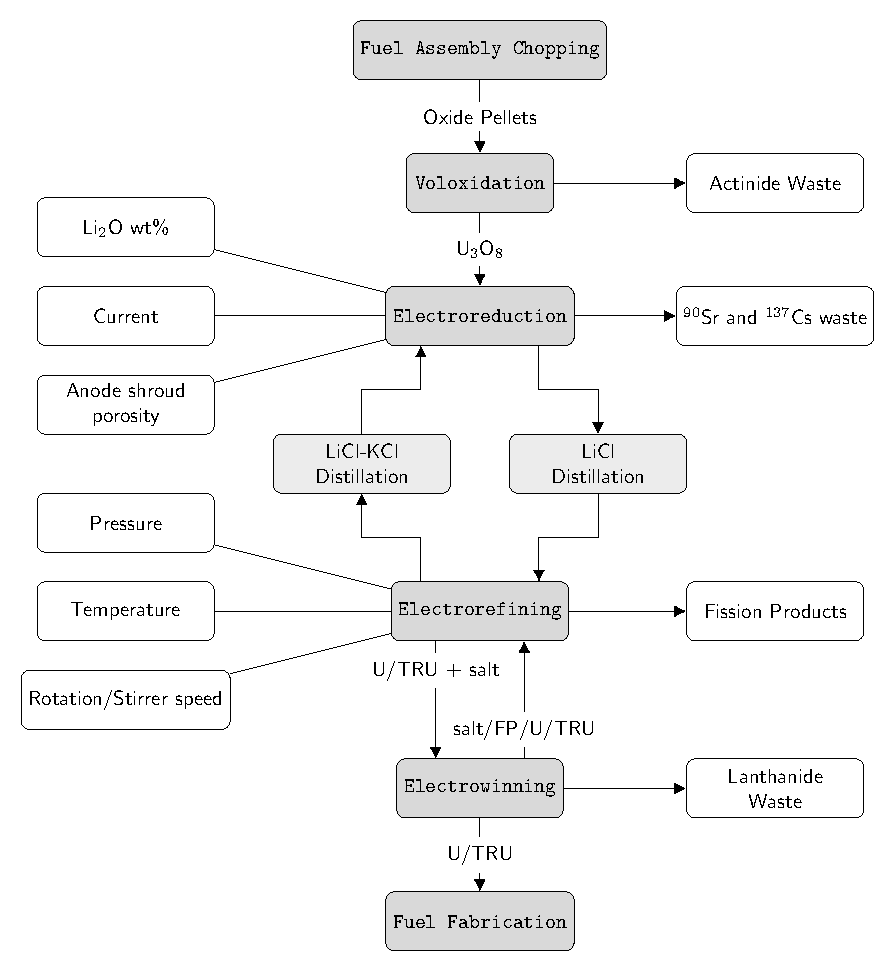
\includegraphics[width=0.9\linewidth]{flowchart}
			\caption{An archetype design flowchart of pyroprocessing facilities.}
			\label{fig:pyre}
		\end{figure}
	\end{column}
\end{columns} 
\end{frame}

